\documentclass[border=4pt]{standalone}
\usepackage{amsmath,amssymb,tikz}
\usetikzlibrary{arrows.meta,calc,matrix,positioning}
\definecolor{figB}{RGB}{31,90,166}\definecolor{figR}{RGB}{176,48,48}\definecolor{figG}{RGB}{46,125,50}\definecolor{figO}{RGB}{214,120,20}
\begin{document}
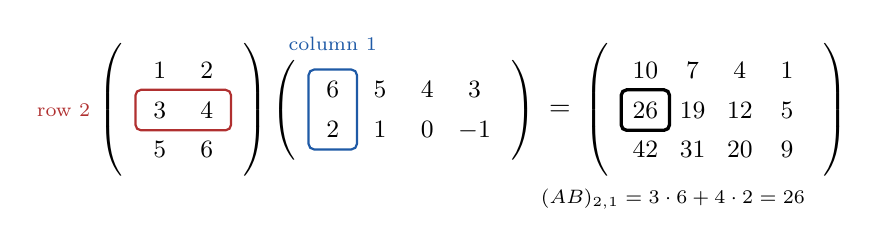
\begin{tikzpicture}[mat/.style={matrix of math nodes,left delimiter=(,right delimiter=),
  nodes={minimum width=0.6cm,minimum height=0.5cm,inner sep=1pt,font=\small},column sep=0pt,row sep=0pt}]
\matrix (A) [mat] at (0,0) {1&2\\3&4\\5&6\\};
\matrix (B) [mat,right=0.75cm of A] {6&5&4&3\\2&1&0&-1\\};
\node[right=0.4cm of B] (eq) {$=$};
\matrix (C) [mat,right=0.4cm of eq] {10&7&4&1\\26&19&12&5\\42&31&20&9\\};
\draw[figR,thick,rounded corners=2pt] (A-2-1.north west) rectangle (A-2-2.south east);
\draw[figB,thick,rounded corners=2pt] (B-1-1.north west) rectangle (B-2-1.south east);
\draw[black,very thick,rounded corners=2pt] (C-2-1.north west) rectangle (C-2-1.south east);
\node[font=\scriptsize,figR,anchor=east] at ($(A-2-1.west)+(-0.45,0)$) {row 2};
\node[font=\scriptsize,figB,anchor=south] at ($(B-1-1.north)+(0,0.12)$) {column 1};
\node[font=\scriptsize,anchor=north] at ($(C-3-1.south)+(0.35,-0.12)$) {$(AB)_{2,1}=3\cdot6+4\cdot2=26$};
\end{tikzpicture}
\end{document}
